\chapter{Validazione preliminare} %\label{1cap:spinta_laterale}
% [titolo ridotto se non ci dovesse stare] {titolo completo}
%


\begin{citazione}
In questo capitolo verrà affrontato il problema della validazione di un motore scacchistico,verranno quindi introdotti i concetti fondamentali alla base della valutazione di un motore e saranno forniti 
degli esempi pratici
\end{citazione}

\newpage
\section*{Validazione preliminare}
Essendo un motore scacchistico un progetto che per sua stessa natura va affrontato con un processo di integrazione continua si rende necessario avere un metodo 
per poter calcolare la nuova forza stimata del motore  ad ogni singolo cambiamento  delle funzioni di ricerca e di valutazione,per assicurarci che i cambiamenti apportati non abbiano reso il motore più debole\footnote{Questo tipo di test è anche detto test di regressione}.
Prima di parlare di "perdere" o "acquisire" forza, è bene introdurre come si quantifica e cosa rappresenta la forza di un motore, il sistema di rappresentazione è mutuato dal sistema utilizzato per classificare i 
giocatori di scacchi da parte delle federazioni scacchistiche, ed è un sistema che prende il nome di ELO, essendo gli scacchi un gioco in cui  rendimento di un giocatore non può essere misurato in maniera assoluta,
ma può solo essere dedotto dai risultati i punteggi hanno significato solo relativamente ai punteggi degli avversari: 
sia la media sia l'intervallo dei punteggi possono essere scelti arbitrariamente. Elo suggerì una scala per cui una differenza di 200 punti significa che il giocatore ha un punteggio atteso di 0,75.
Il punteggio atteso di un giocatore è dato dalla probabilità di vincere, più la metà della probabilità di pareggiare. Quindi un punteggio atteso di 0,75 può rappresentare un 75\% di possibilità di vittoria, 
25\% di sconfitta e 0\% di pareggio, o all'altro estremo 50\% di vittoria, 0\% di sconfitta e 50\% di pareggio.

Se il giocatore A ha una forza reale RA e il giocatore B una forza reale RB, la formula esatta (usando la curva logistica) per calcolare il punteggio atteso del giocatore A è:

\begin{equation}  E_{A}={\frac{{1}}{{1+10^\frac{{{RB} - {RA}}}{{400}}}}} \end{equation}
Similarmente, il punteggio atteso del giocatore B è:
\begin{equation}  E_{B}={\frac{{1}}{{1+10^\frac{{{RA} - {RB}}}{{400}}}}} \end{equation}

Si noti che {\begin{equation}E_{A} +  E_{B}=1 \end{equation}

In pratica, siccome la forza reale di un giocatore è sconosciuta, i punteggi attesi sono calcolati utilizzando i punteggi effettivi dei giocatori. Quando i risultati di un giocatore eccedono il punteggio atteso,
il sistema ELO considera il fatto come evidenza che il punteggio del giocatore è troppo basso: perciò deve essere aggiustato verso l'alto. Se invece i risultati restano sotto il punteggio atteso, 
il punteggio del giocatore viene aggiustato verso il basso. L'idea originale di Elo  ,ancora largamente usata , è quella di un semplice aggiustamento lineare, proporzionale a quanto il giocatore sia stato
sopra o sotto il punteggio atteso. 
Supponendo che il giocatore A abbia un punteggio atteso di ${E_{A}}$ punti, ma abbia ottenuto ${S_{A}}$ punti. La formula per aggiornare il suo punteggio è:

\begin{equation} R_{A}' =R_{A}+K(S_{A}-E_{A})\end{equation}

L'aggiornamento può essere effettuato dopo ogni partita, dopo ogni torneo, o dopo ogni periodo prestabilito. Un esempio può aiutare a comprendere. Supponiamo che il giocatore A abbia un punteggio di 1613, 
e giochi in un torneo con cinque partite. Perde contro un giocatore quotato 1609, pareggia con un giocatore che ha 1477 punti, sconfigge un giocatore con 1388 punti, e uno con 1586, e infine perde con un giocatore 
che ha 1720 punti. Il suo punteggio è $ {(0+0,5+1+1+0)=2,5}$. il suo punteggio atteso, calcolato secondo la formula sopra esposta, avrebbe dovuto essere 
$ (0,506+0,686+0,785+0,539+0,351)=2,867 $. Quindi il suo nuovo punteggio è (1613+32(2,5-2,867))=1601} \cite{itwiki:125247032}.

Come detto precedentemente cosi come per i giocatori umani anche per i motori viene utilizzato il concetto di ELO per la misura delle prestazioni,ci sono però delle differenze pratiche sostanziali,in primis,
a differenza di un giocatore umano , dove " l'hardware" è immutabile, la forza di un motore scacchistico dipende anche dalla potenza di calcolo della macchina sul quale gira, ed in secundis l'elo può dipendere 
da fattori esterni come la gestione del tempo che si ha a disposizione per una mossa,questo è un problema che si applica anche ai giocatori umani ma che fa intrinsecamente parte del loro punteggio in quanto 
un giocatore umano ha libertà di gestire come vuole il proprio tempo, a differenza di un motore scacchistico dove ,soprattutto in motori più basilari, è possibile che il tempo sia gestito in maniera statica.
Per ovviare a questo problematiche ed ottenere una misura di elo significativa è importante uniformare il più possibile la piattaforma sulla quale si effettuano le prove e valutare con attenzione il time control utilizzato.

\begin{figure}[h]
    \centering
    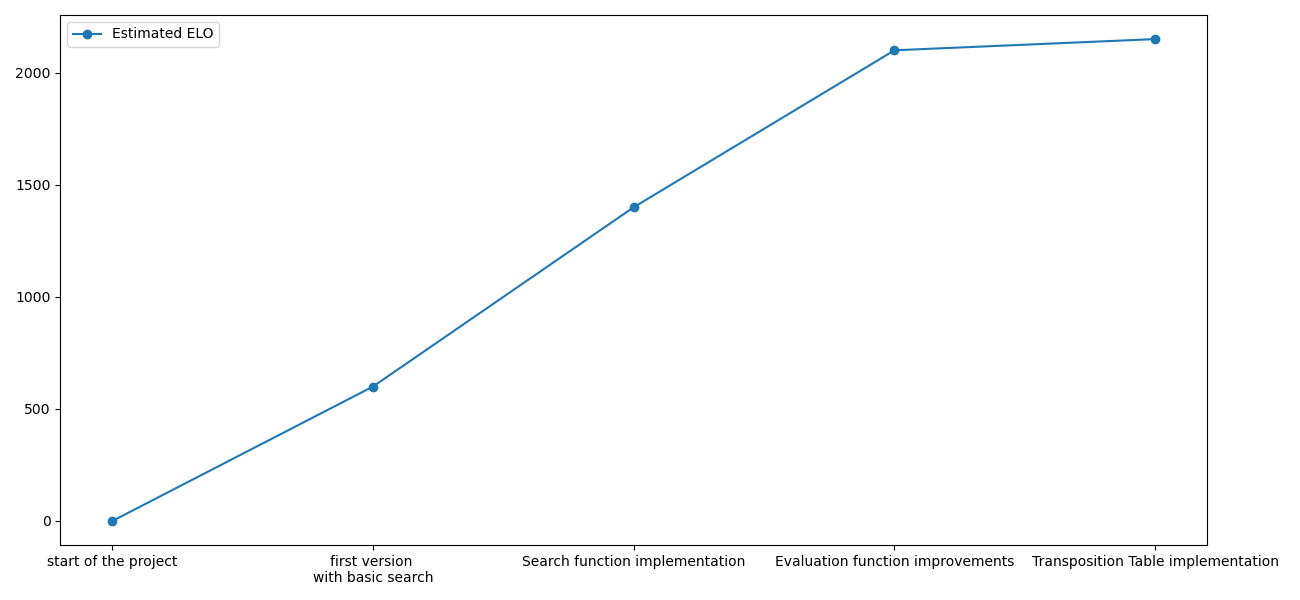
\includegraphics[width=\textwidth]{myplot.png}
    \caption{Valore ELO del motore sviluppato parallelamente a questa tesi ad ogni milestone di sviluppo}
\end{figure}

Oltre al punteggio ELO esistono altre metriche che possono essere utilizzate per analizzare singolarmente alcune delle componenti che compongono un motore,
per la generazione delle mosse abbiamo già visto nel paragrafo \ref{move generation} che è possibile utilizzare la funzione di Perft per valutare le prestazioni di un generatore di mosse,ed essendo la generazione
delle mosse un concetto molto semplice, possiamo seguire un euristica basilare: "più nodi vengono generati al secondo migliore è il generatore",valutare le parti 
di ricerca non è invece altrettanto facile,se è vero che abbiamo un'idea di fondo alla base dell'ottimizzazione della nostra ricerca,ossia "meno nodi vengono esplorati migliore è la funzione di ricerca", è anche vero 
che questo concetto, a differenza di quello della generazione delle mosse, è sottoposto ad ulteriori clausole,vogliamo si che il nostro algoritmo di ricerca esplori meno nodi possibili, ma vogliamo anche che la qualità
delle scelte possibili venga preservata,un numero minore di nodi esplorati quindi, è positivo solo se la forza giocante del nostro motore non diminuisce (o ancor meglio se aumenta), ciò nonostante il variare del numero dei nodi 
può darci un'idea sulla bontà del trade-off ELO/tempo di calcolo necessario ed in generale indicarci se l'approccio che stiamo seguendo meriti o meno ulteriori approfondimenti.
\begin{table}[h]
\begin{center}
    \begin{tabular}{|c|c|c|c|c|} 
     \hline
     Depth & Total Nodes  & $\alpha\beta$ & CE2BIT \\ [0.5ex] 
     \hline
     1 & 20  & 21 & 27 \\ 
     \hline
     2 & 400  &  231 & 110 \\
     \hline
     3 & 8902  &  3346 & 875 \\
     \hline
     4 & 197281  & 18081 &  3142 \\
     \hline
     5 & 4865609  & 138712 & 17430 \\ 
     \hline
     6 & 119060324  & 774756 &   81184 \\
     \hline
    \end{tabular}
    \caption{Confronto tra i numeri esplorati da un semplice algoritmo di ricerca alfa-beta e quelli esplorati dal motore CE2BIT} \label{tab:sometab}
    \end{center}
\end{table}


